\section*{20. Диаграмма Хассе. Определение цепи и антицепи. Теорема о длине наибольшей цепи в ч.у.м. (б/д). Доказательство теоремы на примерах задач о людоедах и числах.}
\textbf{Диаграммой Хассе} называется ориентированный граф без циклов, по которому отношение порядка строится так: $a \leqslant b$, если из a в b идёт ориентированный путь. (см. билет 19) \\ \par

\textbf{Цепь упорядоченного множества $\langle M, \leqslant_M \rangle$} - упорядоченная последовательность элементов $a_1, a_2, \dots, a_n$, для которой $a_i \leqslant_M a_{i+1} $ для всех $1 \leqslant i \leqslant n-1$. \textbf{Антицепь} - набор элементов, никакие два из которых не находятся в отношении $\leqslant_M$. \\ \par
\textbf{Теорема}. Если d длина наибольшей цепи в упорядоченном множестве, то упорядоченное множество можно разбить на d антицепей. \par
\textbf{Задача 6.2 про людоедов} Некоторые людоеды хотят съесть некоторых других людоедов. Известно, что длина наибольшей
цепочки, в которой каждый людоед хочет съесть последующего, равна n (в частности, циклов нет). Докажите, что людоедов можно рассадить в n пещер, в каждой из которых никто никого не хочет съесть. Можно ли гарантированно рассадить их в меньшее число пещер? \par
$\blacktriangle$
Аналогично задаче 6.3, выбираем сначала все минимальные элементы для этого ч.у.м. Каждая следующая пещера: все людоеды, которых хотят съесть только людоеды из предыдущих пещер. Из условия, что максимальная цепь n, мы разбиваем всех великанов на n пещер, в каждой пещере антицепь. При этом гарантированно меньше пещер получить нельзя, рассмотрим пример с n великанами, где каждый великан пронумерован, и хочет съесть всех великанов с номером, большим, чем у него.
$\blacksquare$ \\ \par

\textbf{Теорема}. В упорядоченном множестве из mn + 1 элемента есть цепь длины n + 1 или антицепь из $m + 1$ элемента. \par
\textbf{Задача 6.3 про числа} (а) Докажите, что среди 36 различных натуральных чисел или найдется 6 чисел, среди которых ни одно не делится на другое, или найдется 8 чисел, которые можно выстроить в цепь, где каждое число делится на следующее. (б) Верен ли аналогичный факт для целых чисел? \par
$\blacktriangle$
(а) Пусть не найдётся ни цепь длины 8, ни антицепь длины 6. Тогда возьмём все числа, которые в данном ч.у.м. являются минимальными. Очевидно, что количество таких чисел $\leqslant 5$. Последовательно будем выбирать множества чисел, которые делятся только на числа из предыдущих множеств; получим следующую схему: \\ 
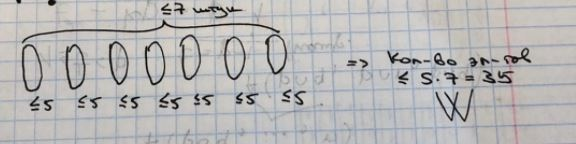
\includegraphics{images/20} \\

Нашли противоречие. Значит, начальное утверждение неверно. \\
(б) Формально, делимость среди целых чисел не является ч.у.м., т.к. нарушена антисимметричность => теорема не применима с её доказательством. Однако мы можем доопределить целые числа до ч.у.м.: будем считать, что -7 делится на 7, но не наоборот. Тогда делимость на таких целых числах будет ч.у.м. и можно применить теорему (аналогичные рассуждения из пункта а)
$\blacksquare$